\begin{problem}{稻妻的谜题}{standard input}{standard output}{1.5 seconds}{256 megabytes}

神樱大祓任务中,巫女花散里带旅行者来到井底。

在这里有多个祝祷座,有唯一一个祝祷座上面勾玉数量为$1$,这个祝祷座不可修改,其他的祝祷座可以通过修改使得它上面的勾玉数量为任何大于等于$2$的整数。此外有一个鸟居,上面有一幅关于谜题的图案。

\begin{center}
  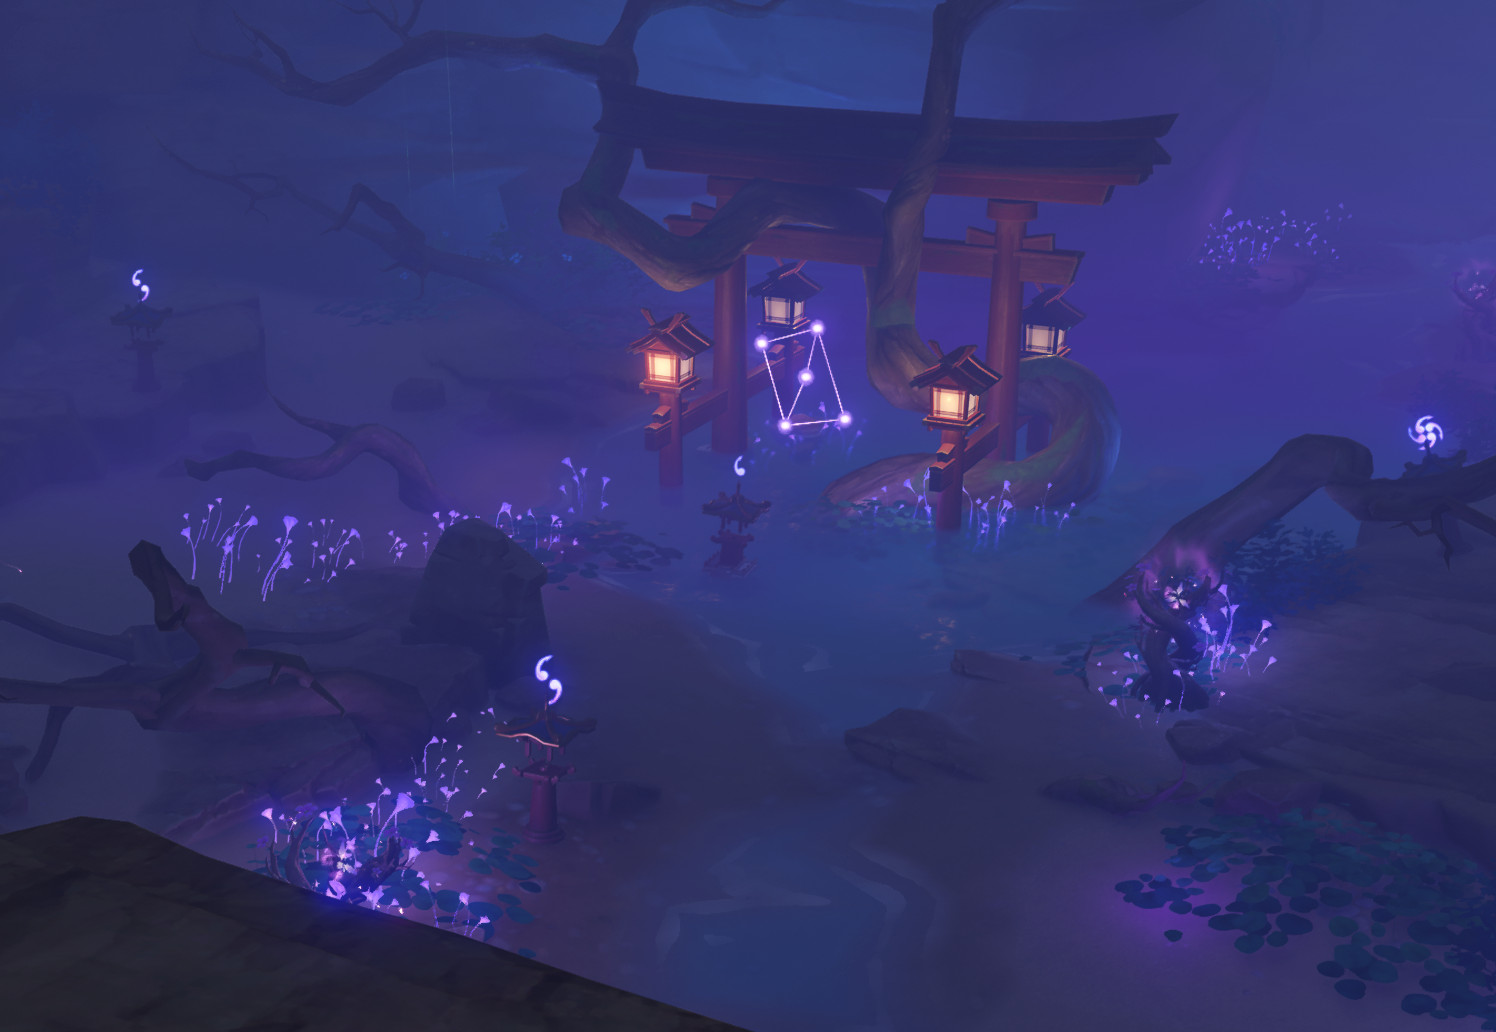
\includegraphics[scale=0.25]{puzzle.jpg} \\
  \small{神樱大祓任务}
\end{center}

修改完成后,旅行者回到勾玉数量为$1$的祝祷座进行祝祷,此时,所有勾玉数量为$1$的祝祷座会连接所有勾玉数量为$2$的祝祷座,所有勾玉数量为$2$的祝祷座会连接所有勾玉数量为$3$的祝祷座,以此类推,所有勾玉数量为$n$的祝祷座会连接所有勾玉数量为$n + 1$的祝祷座。

祝祷后,祝祷座之间的连接情况必须于鸟居上的图案完全一致,即两个祝祷座图案上连接,旅行者祝祷后也必须连接,反之亦然。鸟居上的图案没有勾玉数量,并且保证图案上所有的祝祷座直接或间接与勾玉数量为$1$的祝祷座相连。注意连接是没有方向的。

因为旅行者需要多次在此任务中解出类似谜题,他/她希望你编写一个程序帮他/她解决这个谜题,或者表明这个谜题无解。

\InputFile
两个整数$n$、$m$,图案上祝祷座的数量和连接的数量,其中勾玉数量为$1$的祝祷座为$1$号。($2 \le n \le 10^5$、$1 \le m \le \min {\{\dfrac{n(n - 1)}{2}, 10^5\}}$)
接下来$m$行,每行两个整数$u$、$v$,表示$u$与$v$相连。($1 \le u < v \le n$)

\OutputFile
如果有解,输出``YES'',接下来一行$n - 1$个整数,表示除了$1$号祝祷座以外每个祝祷座上勾玉的数量。

如果无解,输出``NO''。

不区分大小写。

\Examples

\begin{example}
\exmpfile{example.01}{example.01.a}%
\exmpfile{example.02}{example.02.a}%
\exmpfile{example.03}{example.03.a}%
\end{example}

\end{problem}

